\subsection{Network and observation campaign}
\label{sec:results-network}

\begin{figure}[t]
  \centering
  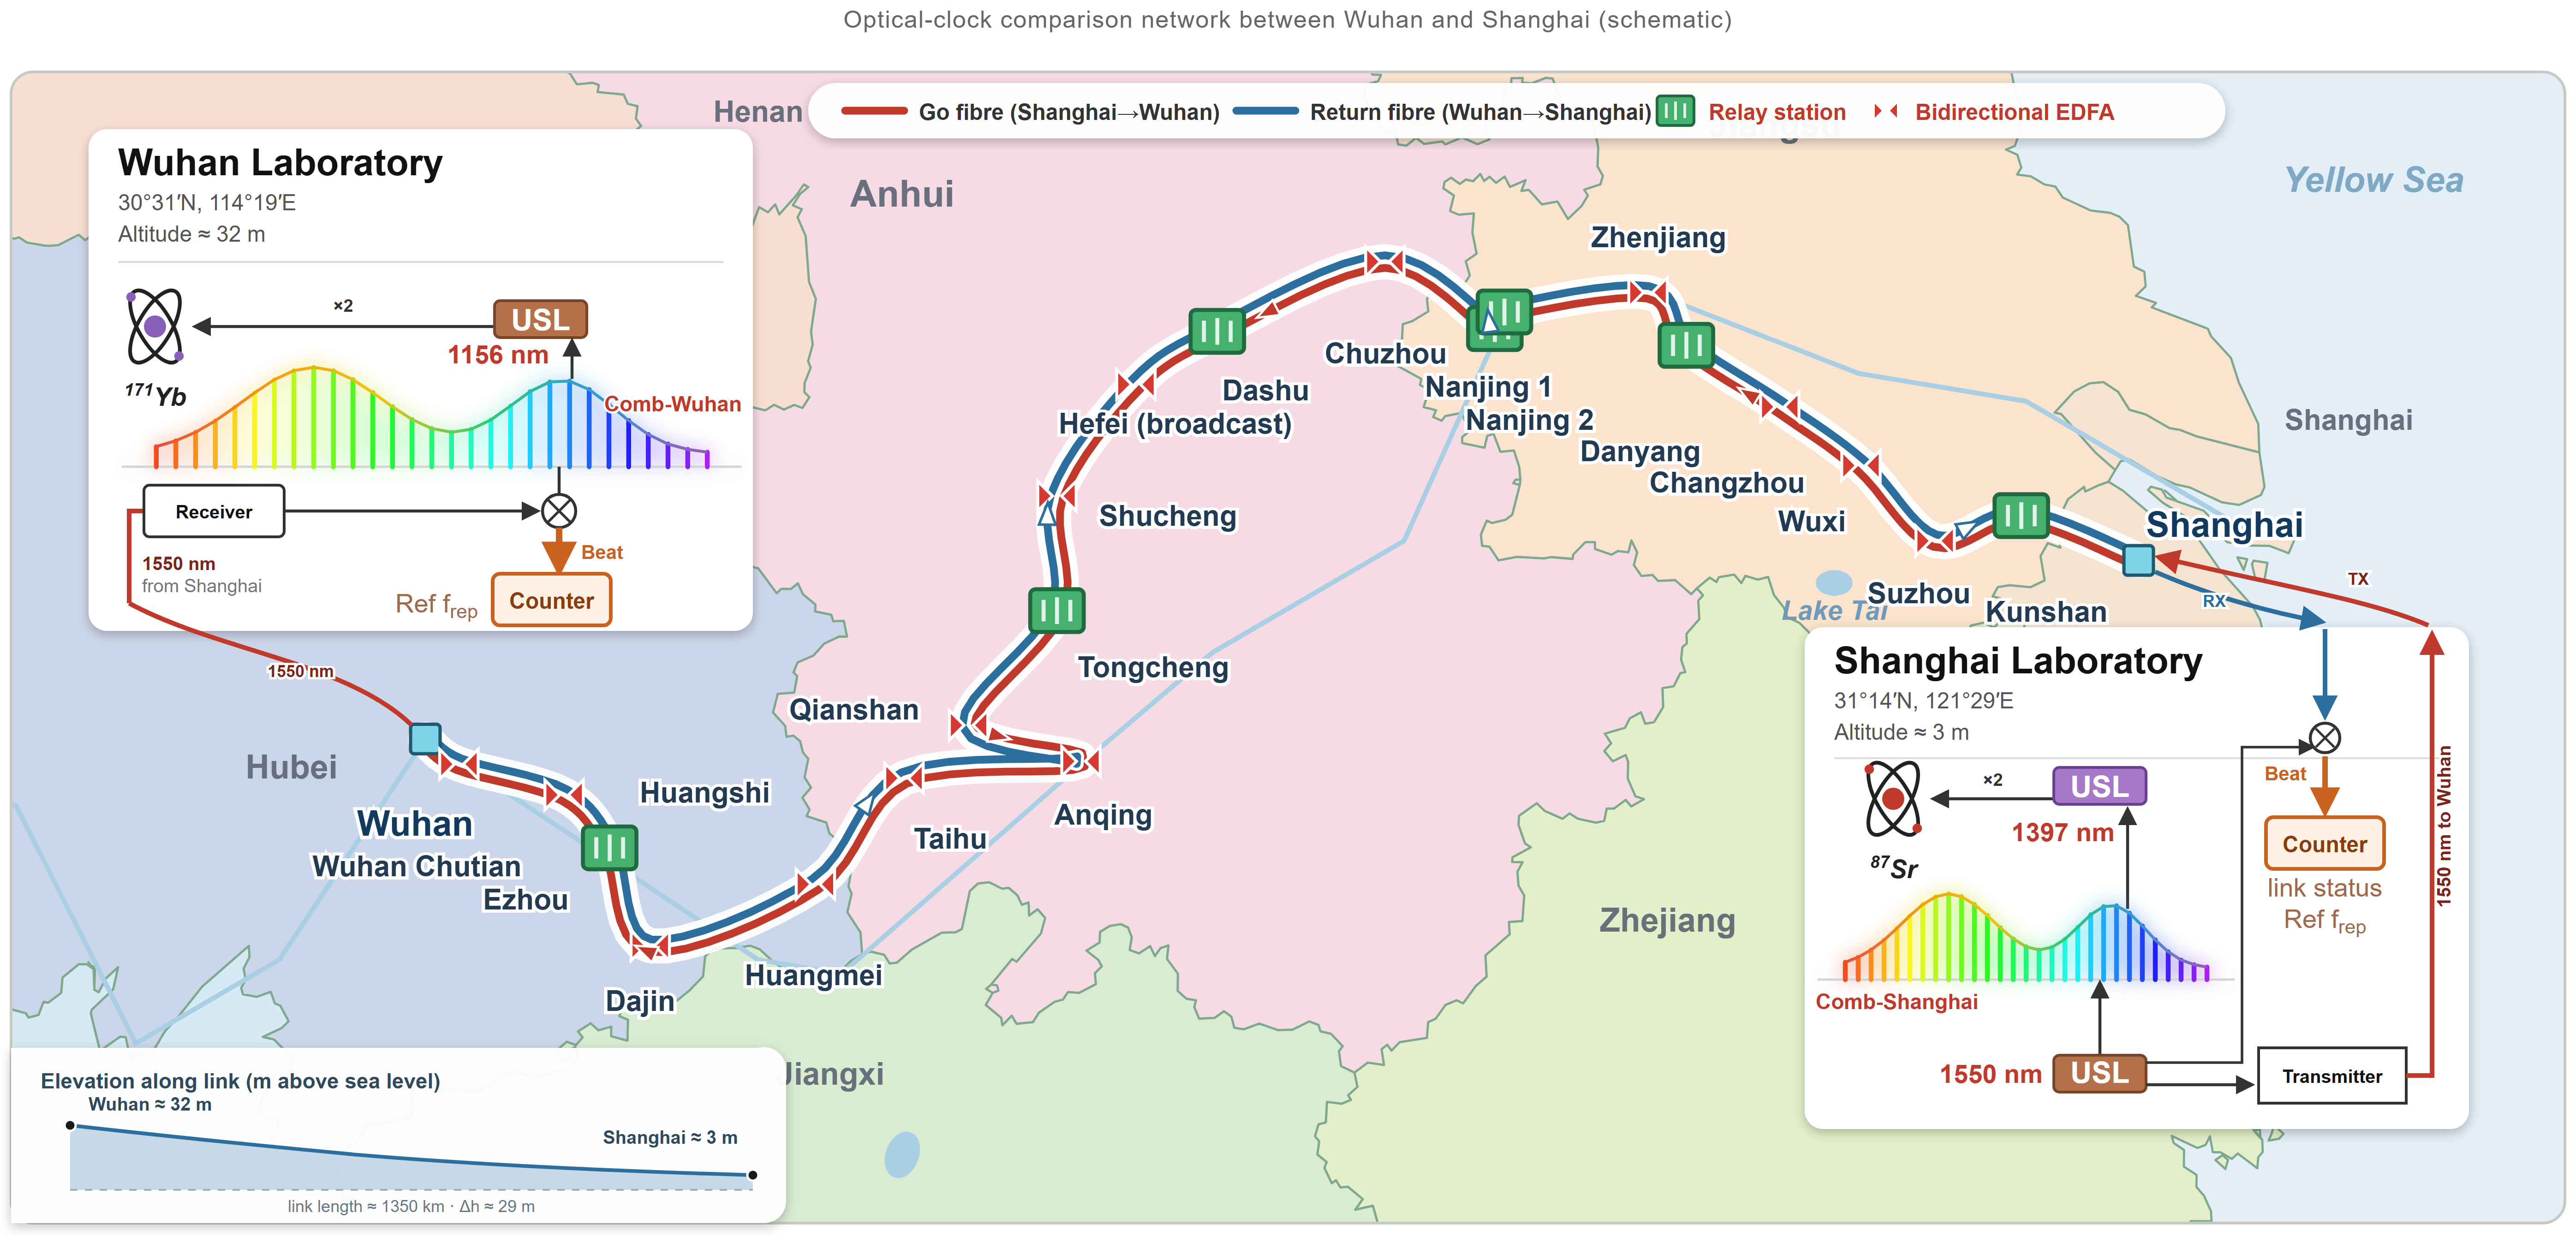
\includegraphics[width=\linewidth]{figs/fig1_network.png}
  \caption{The two-clock network. An IAPMST ytterbium clock in Wuhan and
  a USTC strontium clock in Shanghai are connected by a phase-stabilized
  \qty{1550}{nm} fiber link. Relay stations along the route carry
  erbium-doped fiber amplifiers and fiber-noise-cancellation loops.}
  \label{fig:network}
\end{figure}

Figure~\ref{fig:network} shows the two-clock network. An ytterbium (Yb)
lattice clock at IAPMST~\citep{zhu2026yb} in Wuhan (systematic
uncertainty $\uYbE\times10^{-18}$) and a strontium (Sr) lattice clock
at USTC~\citep{jia2026sr} in Shanghai ($\uSrE\times10^{-18}$) are
separated by $\siteKm$\,km and compared through a $\fibreKm$\,km
phase-stabilized fiber link ($\roundKm$\,km loop-back) on a commercial
telecom network used non-exclusively, with the carrier transmitted from
Shanghai to Wuhan on the ITU-T 100\,GHz DWDM channel C34
(\qty{1550.12}{nm}, \qty{193.4}{THz}). The link extends the
field-deployed link of ref.~\citep{chen2026dissemination}, using the
same cascaded fiber-noise-cancellation technique; its added instability
stays below the clock noise for averaging times beyond $100$\,s.

Both combs are self-referenced and phase-locked to the local clock
signal, and all other frequencies in the chain derive from the two
clock transitions through fixed factor-of-two relations
(698/1397 nm on the Sr side; 578/1156 nm on the Yb side), so the two
clocks are the system's only independent frequency sources. The
recorded quantity is the out-of-loop beat between the received carrier
and the local Yb-referenced comb, sampled every second and converted to
fractional units by normalizing to the carrier frequency $F_{1550}$
(\qty{1550.12}{nm}); the fiber loop-back is monitored out of
loop throughout. The geopotential difference between the two clocks was
measured by spirit leveling to be
$\dW = \dWVal \pm \dWUnc~\mathrm{m^{2}\,s^{-2}}$ (see Methods). Each
retained segment yields a frequency-ratio estimate through the fixed
frequency-chain relations (see Methods).

\subsection{Clock-ratio determination}
\label{sec:results-ratio}

Over two months (\nDays~days) the two clocks and their transfer chains
ran synchronously for a total of \nHours~effective hours, recorded as
\nSeg~jump-free segments. The results are presented in
Figure~\ref{fig:ratio}.

\begin{figure}[t]
  \centering
  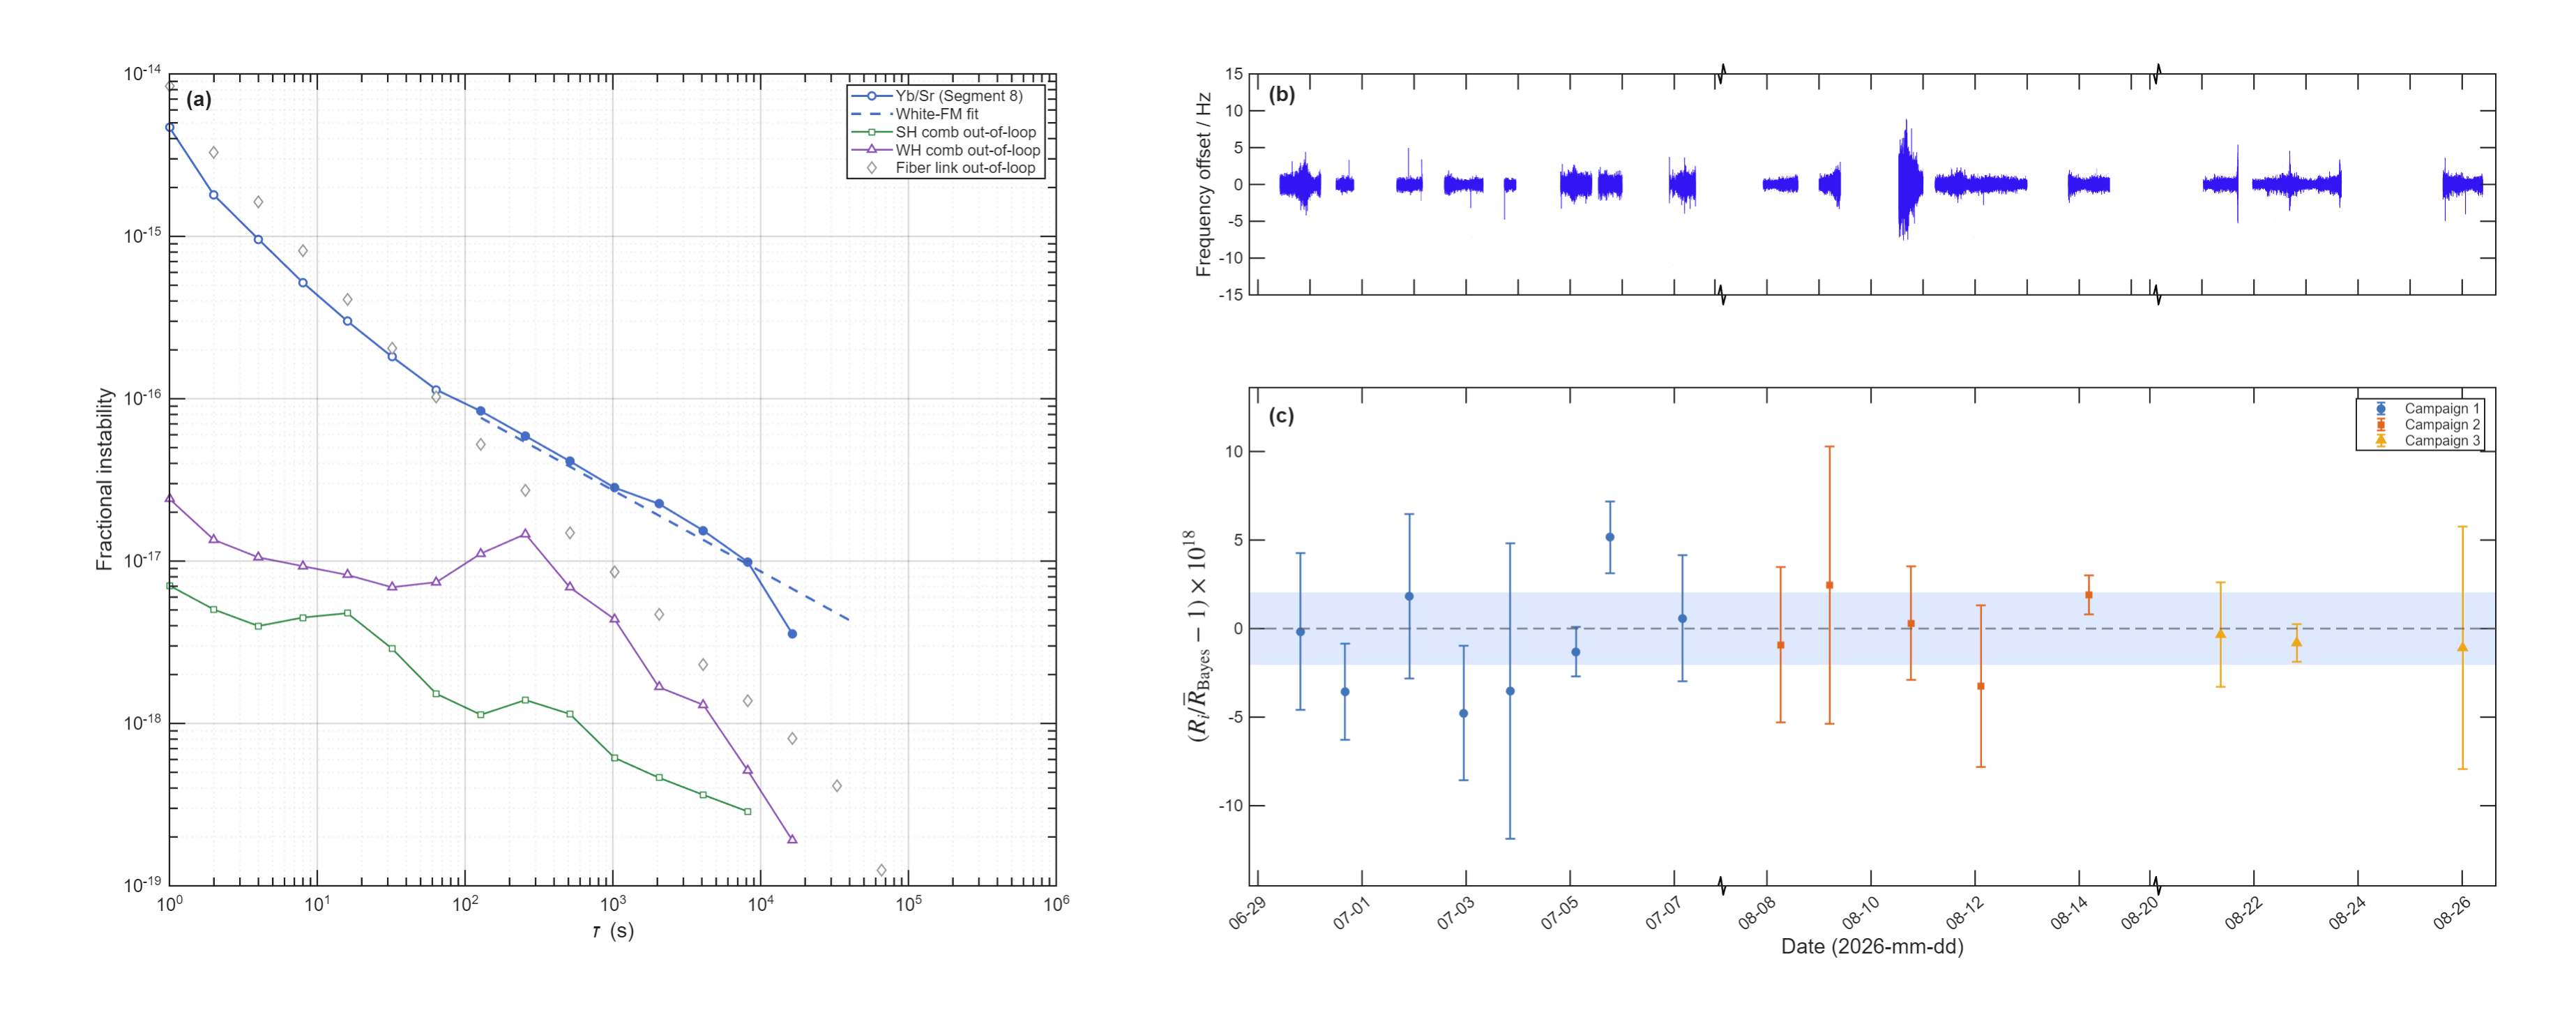
\includegraphics[width=\linewidth]{figs/fig2_ratio.pdf}
  \caption{Frequency-ratio measurement results. (a) Fractional
  instability of a representative segment (Yb/Sr, segment 8); the
  points are the overlapping Allan deviation at different averaging
  times $\tau$. The solid line is a white-frequency-noise model
  $\sigma_y(\tau) = \sigma_0/\sqrt{\tau/\mathrm{s}}$; the statistical
  uncertainty is the last computable point of the stability record,
  without extrapolation. The gray markers are the out-of-loop
  instabilities of the two frequency combs (SH, WH) and of the fiber
  link. (b) Per-campaign ratio measurements as fractional deviations
  from the final reported value, with error bars from the procedure in
  (a). (c) The same deviations by campaign date.}
  \label{fig:ratio}
\end{figure}

In Figure~\ref{fig:ratio}a, the overlapping Allan deviation of the
fractional ratio for a representative segment follows a white
frequency noise law $\sigma_y(\tau) = \sigma_0/\sqrt{\tau/\mathrm{s}}$
over most of the record. The statistical uncertainty of each segment
is obtained from the last computable point of its stability record
rather than by extrapolating the white-noise fit to the segment
duration; together with the segment mean, this provides one data point
per segment, as plotted in Figure~\ref{fig:ratio}b,c.

We determine the Yb/Sr frequency ratio from the \nSeg~segments. Each
segment yields a ratio estimate with its own statistical uncertainty
(Methods). The segment
estimates are consistent with their individual uncertainties, as
quantified by the combination statistics in
Table~\ref{tab:estimators}. Following recent ratio
comparisons~\citep{pizzocaro2026european, aeppli2026nist}, we combine
the segments with a random-effect model that admits a common excess
scatter~\citep{birge1932errors, mandel1970interlaboratory}, and
evaluate three estimators (Table~\ref{tab:estimators}). The three
agree at the $10^{-18}$ level; the Bayesian random-effect estimate,
which carries the largest standard uncertainty, is reported as the
primary value,
\begin{equation}
  \mathrm{Yb/Sr} = \Rheadline,
\end{equation}
with statistical uncertainty $\uStatE\times10^{-18}$ (see Methods for
the model-limited segments).

\begin{table}[t]
  \centering
  \caption{Statistical combination of the \nSeg~segment ratios.
  WLS denotes weighted least squares with inverse-variance weights
  $w_i = 1/u_i^2$; $\xi$ is the inferred common excess scatter. The
  weighted combination yields $\chi^2_{\rm red} = \chiRed$ for
  $\dofV$ degrees of freedom ($p = \pChi$) and a Birge ratio of
  $\birgeRatio$. All three estimators agree at the $10^{-18}$ level;
  the Bayesian random-effect value carries the largest standard
  uncertainty and is reported as the primary result.}
  \label{tab:estimators}
  \begin{tabular}{lS[table-format=1.21]S[table-format=1.3]S[table-format=1.2]}
    \toprule
    Estimator & {Yb/Sr} & {$u$ ($10^{-18}$)} & {$\xi$ ($10^{-18}$)} \\
    \midrule
    WLS (inverse variance)   & \RwlsRawT & \uWlsE & {---} \\
    Mandel--Paule            & \RmpRawT & \uMpE & \xiMpE \\
    Bayesian random effect   & \RbayesRawT & \uStatE & \xiBayesE \\
    \bottomrule
  \end{tabular}
\end{table}

\subsection{Uncertainty budget}
\label{sec:results-budget}

Beyond the statistical uncertainty of the ratio combination, the
comparison carries several systematic contributions: the published
evaluations of the two clocks, the geodetic determination of the
gravitational-potential difference between the sites, and the
residuals of the transfer subsystems. We discuss each in turn and
combine them into the total standard uncertainty
(Table~\ref{tab:budget}).

The Sr clock contributes $\uSrE\times10^{-18}$ from its published
systematic evaluation~\citep{jia2026sr}, and the Yb clock
$\uYbE\times10^{-18}$~\citep{zhu2026yb}. The static
gravitational-potential term is the leveling uncertainty
$\dWUnc~\mathrm{m^2\,s^{-2}}$ converted to fractional frequency as
$u(\dW)/c^2$, giving $\uStaticE\times10^{-18}$; this is the same
leveled geopotential difference already applied as the static
correction (Section~\ref{sec:results-network}). The frequency
conversion stages each contribute $\uLinkE\times10^{-18}$ and
$\uCombE\times10^{-18}$ from the frequency-reference settings of the
frequency conversion.

The time-varying gravitational redshift is more involved. The tide
series used in this analysis was computed with the public software
ETideLoad4.5 (Earth Tide, Load Effect and Deformation Monitoring
Computation)~\citep{zhang2026etideload}, which implements the
geophysical models and numerical standards of the IERS Conventions
(2010)~\citep{iers2010conventions}. Solid Earth
and ocean tides, together with atmospheric, hydrological and
non-tidal ocean loading, move the local potential by amounts reaching
the $10^{-18}$ level over the campaign~\citep{agnew2015tides,
voigt2016timevariable, denker2018geodetic}, and no single tide model
accounts for all of them consistently. Attempting to correct the beat
record with the supplied tide series degrades the fit rather than
improving it: the reduced chi-square of the combination rises from
$\tidalChiRaw$ to $\tidalChiTheory$ (fixed theoretical amplitude) or
$\tidalChiEmp$ (fixed historical amplitude) when the template is
applied before the ratio inversion, evidence that the model is
incomplete at this level. We therefore treat the time-varying term as
an uncertainty rather than a correction. Its magnitude is estimated
by the method of the present analysis: the ratio combination is
repeated with the tide template applied at a fixed amplitude, and the
resulting Bayesian center shift,
$\tidalShiftEmpE\times10^{-18}$, is adopted (rounded) as the
uncertainty item $\uTidalE\times10^{-18}$. A physically complete,
data-consistent treatment of time-dependent gravity is deferred to
future work.

Combining the statistical and systematic components in quadrature
gives the total standard uncertainty
$\uTotalShort\times10^{-18}$; the reported ratio is therefore
\begin{equation}
  \mathrm{Yb/Sr} = \Rheadline(\RheadlineUnc),
\end{equation}
where the parenthesized digits are the total standard uncertainty in
the last two decimal places of the value.

\begin{table}[t]
  \centering
  \caption{Uncertainty budget of the Yb/Sr frequency-ratio
  measurement. The time-varying gravitational-redshift term is carried
  as an uncertainty item and is not applied as a correction to the
  central value. Components are treated as independent.}
  \label{tab:budget}
  \begin{tabular}{lS[table-format=1.3]}
    \toprule
    Component & {Contribution ($10^{-18}$)} \\
    \midrule
    Statistical (Bayesian random effect) & \uStatE \\
    Sr systematics                       & \uSrE \\
    Yb systematics                       & \uYbE \\
    Static gravitational potential       & \uStaticE \\
    Fiber link                           & \uLinkE \\
    Frequency comb                       & \uCombE \\
    Time-varying redshift                & \uTidalE \\
    \midrule
    Total (quadrature)                   & \uTotalE \\
    \bottomrule
  \end{tabular}
\end{table}
